% This is samplepaper.tex, a sample chapter demonstrating the
% LLNCS macro package for Springer Computer Science proceedings;
% Version 2.20 of 2017/10/04
%
\documentclass[runningheads]{llncs}
\usepackage[english]{babel}
% for in-text and parentheis citations (works with technopress bib style)
\usepackage[round, authoryear]{natbib}
% for hyperlinking cross-references
\usepackage{hyperref}
% For figures
\usepackage{graphicx}
% For block quotes (see https://tex.stackexchange.com/questions/325695/how-to-style-blockquote and https://tex.stackexchange.com/questions/140300/how-to-prevent-pagebreak-in-quote-environment)
\usepackage{etoolbox}
\usepackage{setspace} % for \onehalfspacing and \singlespacing macros

%% for multiple comma-separated footnotes (see https://tex.stackexchange.com/questions/40072/incompatibility-between-footmisc-option-multiple-and-hyperref/62091#62091)
%! suppress = DiscouragedUseOfDef
\let\oldFootnote\footnote
\newcommand\nextToken\relax
\renewcommand\footnote[1]{\oldFootnote{#1}\futurelet\nextToken\isFootnote}
\newcommand\isFootnote{\ifx\footnote\nextToken\textsuperscript{,}\fi}

% For block quotes
\newenvironment{nbquote} {\quote\interlinepenalty=10000 } {\endquote}
\AtBeginEnvironment{nbquote}{\par\singlespacing\small}

% Used for displaying a sample figure. If possible, figure files should
% be included in EPS format.
%
% If you use the hyperref package, please uncomment the following line
% to display URLs in blue roman font according to Springer's eBook style:
% \renewcommand\UrlFont{\color{blue}\rmfamily}

\begin{document}
%
    \title{CS 715 Seminar Thesis}
    \subtitle{Linked Data on the Web}
%
%\titlerunning{Abbreviated paper title}
% If the paper title is too long for the running head, you can set
% an abbreviated paper title here
%
    \author{Lukas M. Loos}
%
%\authorrunning{F. Author et al.}
% First names are abbreviated in the running head.
% If there are more than two authors, 'et al.' is used.
%
    \institute{University of Mannheim}
%
    \maketitle              % typeset the header of the contribution
%
    \begin{abstract}
        The abstract should briefly summarize the contents of the paper in
        150--250 words.

    \end{abstract}
%
%
%


    \section{Available Data}

    \subsection{Linked Open Data}
    When \citet{berners2001semantic} introduced the idea of the semantic web as an evolution of the original document web, their vision was to allow agents to infer the meaning of instances and their relationships published in datasets on the web.
    This is enabled by assigning instances and relations to URIs from standardized vocabularies, making their meaning no more limited to the dataset's scope but globally valid.
    The semantic web relies on various technological standards of which some were specifically developed for it and others already existed.
    Firstly, just like the document web, it relies on HTTP for data transmission.
    RDF~\citep{RDF}, a standard published by the World Wide Web Consortium (W3C) is the recommended language for transferring linked data and describes datasets as collections of triples consisting of subjects, predicates, and objects.
    Vocabularies for linked data are organized in ontologies, defined in the standards RDFS~\citep{RDFS} and OWL~\citep{OWL}.
    Finally, SPARQL~\citep{SPARQL}, another standard by the W3C is a query language that can be used to query linked datasets.

    \subsection{Linked Open Data Cloud}
    Probably the most prominent service around linked open data is the Linked Open Data Cloud (LOD-cloud)
    \footnotemark{} (see Figure~\ref{fig:lod_cloud}).
    The LOD-cloud is a diagram visualizing linked open datasets and their interconnections.

    \begin{figure}[ht]
        \centering
        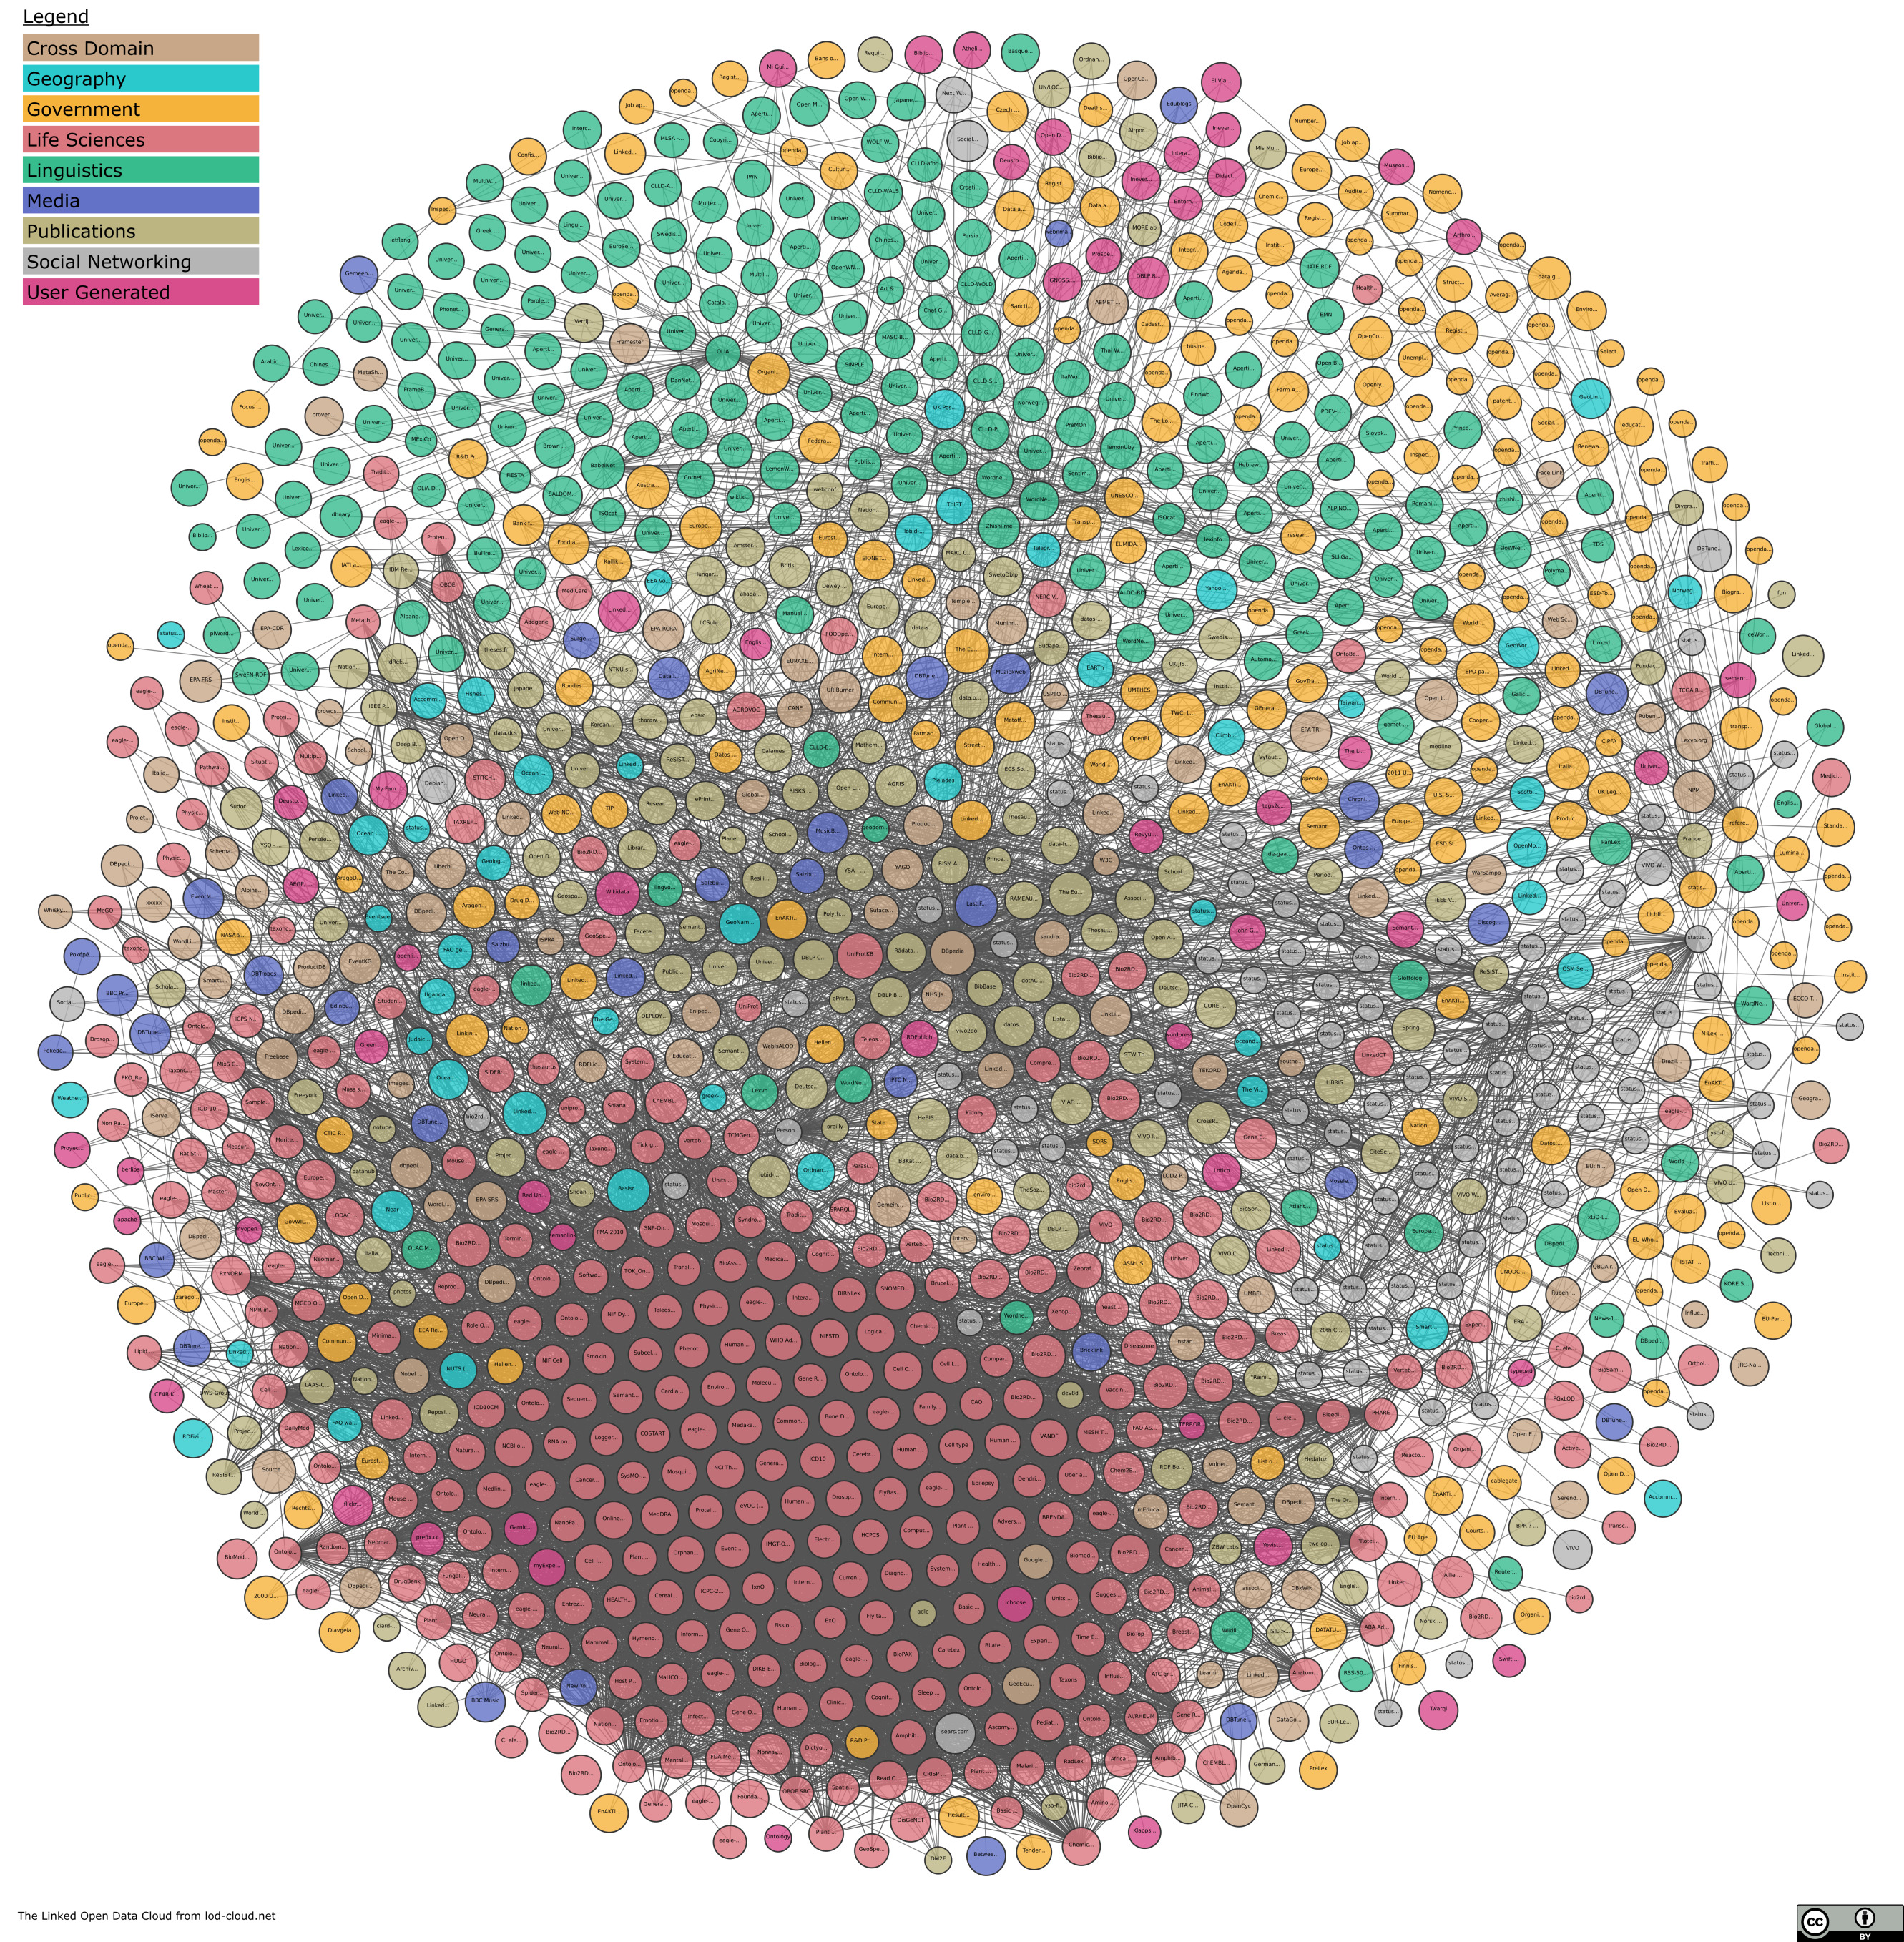
\includegraphics[width=\textwidth]{figures/lod-cloud-sm}
        \caption{The LOD-cloud\protect\footnotemark[\value{footnote}]}
        \label{fig:lod_cloud}
    \end{figure}

    For a dataset to be included, it has to meet certain requirements.
    For example, instances have to be annotated with URIs that resolve to RDF data, the dataset must contain at least 1000 triples, and it has to be connected via RDF links to datasets in the diagram with at least 50 links.
    The LOD-cloud also provides metadata about the datasets.
    For example, it divides the datasets into different domains, like Media, Government, Publications, Social Networking, or Life Sciences.
    As of May 2021 this catalogue contained 1301 datasets and has become the subject of multiple investigations~\citep{debattista2019lod, kamdar2019enabling, schmachtenberg2014adoption}.

    \subsection{Life Sciences Linked Open Data Cloud}
    In this thesis, I will focus on datasets from the life sciences domain, colored red in Figure~\ref{fig:lod_cloud}.
    This part of the LOD-cloud is often also referred to as life-sciences LOD-cloud (LSLOD-cloud) and is depicted in more detail in Figure~\ref{fig:lslod_cloud}.

    \begin{figure}[ht]
        \centering
        \includegraphics[width=\textwidth]{figures/life-sciences-lod}
        \caption{The LSLOD-cloud\protect\footnotemark[\value{footnote}]}
        \label{fig:lslod_cloud}
    \end{figure}
    \footnotetext{The Linked Open Data Cloud, https://lod-cloud.net/, (Accessed on 01/06/2022)}

    Biomedical researchers have already been adopting semantic web technologies in their early stages~\citep{ashburner2000gene, bodenreider2004unified, wang2005xml}, motivated by a problem that still exists in the domain and was addressed by Vijay Bulusu, head of data and digital innovation at company Pfizer:
    \begin{nbquote}
        Vijay Bulusu opened his plenary session at the Bio-IT World Conference \& Expo last week by asking the audience whether - if given \$1 million to spend - they'd buy a machine learning platform or improve the quality of their data.
        Nearly everyone voted for improving data quality.
        Bulusu was pleased.
        Life sciences doesn't really have a big data problem, he explained.
        It has a "lots-of-small-data problem," and data should be our focus~\citep{Pfizer}.
    \end{nbquote}

    Datasets in the LSLOD-cloud describe entities such as molecules (e.g., drugs or proteins) and their characteristics, biological pathways, organs, or diseases~\citep{bodenreider2008biomedical}.
    In their attempt to implement a query engine that was supposed to make SPARQL endpoints of LSLOD datasets more accessible, \citet{kamdar2014roadmap} catalogued linked concepts and properties from 137 public SPARQL endpoints to map concepts and properties to so-called Query Elements.
    Figure~\ref{fig:lslod_entities} gives an overview of the number of entities from the datasets linked to different types of Query Elements.

    \begin{figure}[ht]
        \centering
        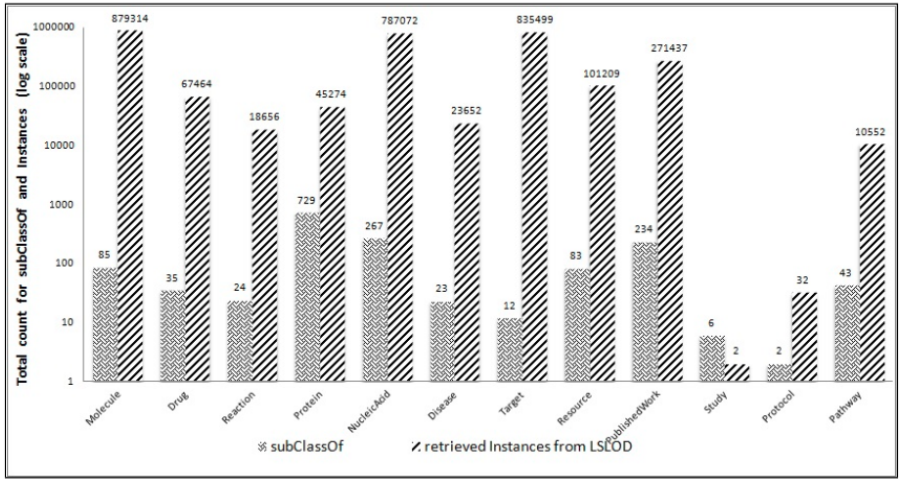
\includegraphics[width=\textwidth]{figures/lslod_entities}
        \caption{Representation of different types of entities in LSLOD Dataset~\citep{kamdar2014roadmap}.}
        \label{fig:lslod_entities}
    \end{figure}
    \footnotetext{The Linked Open Data Cloud, \url{https://lod-cloud.net/}, (Accessed on 01/06/2022)}


    \section{Data Publishers}
    A very large part of the datasets in the LSLOD-cloud are published two projects:
    NCBO BioPortal~\citep{BioPortal} and Bio2RDF~\citep{Bio2RDF}.

    \subsection{BioPortal}
    BioPortal is a project funded by the National Institute of Health (NIH) and provides centralized access to a collection of biomedical ontologies.
    Since the provided datasets are ontologies, they do not contain any instance data, but define classes and properties that can be used as vocabularies to type instances in other datasets.
    In January 2022, the collection consisted of 953 ontologies, containing $13,732,155$ classes, and $36,286$ properties\footnote{NCBO BioPortal, \url{https://bioportal.bioontology.org/}, (Accessed on 01/08/2022)}.
    Only a subset of these ontologies are registered in the LSLOD-cloud.
    BioPortal is not the original publisher of the provided ontologies, but rather provide unified access to ontologies from different sources like SNOMED CT\footnote{SNOMED International, \url{https://www.snomed.org/}, (Accessed on 01/08/2022)}, a large, general purpose clinical ontology or RxNORM\footnote{RxNorm, \url{https://www.nlm.nih.gov/research/umls/rxnorm/index.html}, (Accessed on 01/08/2022)}, an ontology about clinical drugs which is part of the UMLS, another project related to the NIH that also provides linked data, however not using semantic web technologies.

    \subsection{Bio2RDF}
    Bio2RDF is an open source project maintained by Maastricht University and Universit\'e Laval and claims to provide the largest network of linked data in the domain of life sciences\citep{Bio2RDF_Github}.
    Like BioPortal, Bio2RDF are not the authors of the datasets they publish, but rather translated datasets from sources such as DrugBank\footnote{DrugBank Online, \url{https://go.drugbank.com/}, (Accessed on 01/08/2022)} or FarmGKB\footnote{PharmGKB, \url{https://www.pharmgkb.org/}, (Accessed on 01/08/2022)} into RDF\@.
    In contrast to BioPortal however, Bio2RDF provides LSLOD datasets with instance data and not ontologies.

    \subsection{Other LSLOD Publishers}
    An example for a publisher of LSLOD who is also the author of the provided datasets is the RDF Platform of the European Bioinformatics Institute (EBI)\footnote{RDF Platform, \url{https://www.ebi.ac.uk/rdf/}, (Accessed on 01/09/2022)}.
    The EBI is part of the European Molecular Biology Laboratory (EMBL), a research organization, funded by the governments of its 27 member states and provides SPARQL access points to several databases with biomedical data.

    Pharmaceutical companies, certainly among the main players in the biomedical domain have a seemingly conflicting relation to linked open data.
    I researched the practices of data sharing of the 3 largest companies by market capitalization\footnote{Largest pharma companies by market cap, \url{https://companiesmarketcap.com/pharmaceuticals/largest-pharmaceutical-companies-by-market-cap/}, (Accessed on 01/09/2022)}, namely, Johnson \& Johnson, Roche and Pfizer.
    These companies are in possession of large amounts of data of immense public value, and while they do claim to share data from clinical trials over various channels\footnote{Roche - Our commitment to data sharing, \url{https://www.roche.com/research_and_development/who_we_are_how_we_work/research_and_clinical_trials/our_commitment_to_data_sharing.htm}, (Accessed on 01/09/2022)}\footnote{Advancing Clinical Trial Data Sharing Through the Yale University Open Data Access Project | Johnson \& Johnson, \url{https://www.jnj.com/innovation/yale-open-data-access-project}, (Accessed on 01/09/2022)}\footnote{Data Access Requests | Pfizer, \url{https://www.pfizer.com/science/clinical-trials/trial-data-and-results/data-requests}, (Accessed on 01/09/2022)}, none of them seem to do so via linked open data.
%    todo: add something about how they are using lod anyways
%    todo: Johson & Johnson took part in W3C Linking Open Drug Data initiative 16. Jentzsch, A. et al. Linking Open Drug Data. In I-SEMANTICS (2009). Drug data integration project

    \section{Change of LSLOD over the Last Years}
    \subsection{Datasets in the LOD-cloud}
    \citet{schmachtenberg2014adoption} compared the adoption of LOD best practices in LOD-cloud datasets in 2011 and 2014.
    I augmented their data with LOD-cloud metadata from the years 2018--2021, retrieved from archive.org\footnote{Internet Archive: Wayback Machine, \url{https://archive.org/web/}, (Accessed on 01/09/2022)}.
    Figure~\ref{fig:lod-cloud-change} shows the change in the number of datasets in different domains over the recent years.
    While especially in the life-sciences domain, the number has been increasing relatively fast until 2018, this trend seems to have slowed down in the recent years.
    This trend seems not to exclusively affect the domain of life-sciences.
    The domain of linguistics seems to show a similar trend and other domains' growth (e.g., publications) has stopped already much earlier.

    \begin{figure}[ht]
        \centering
        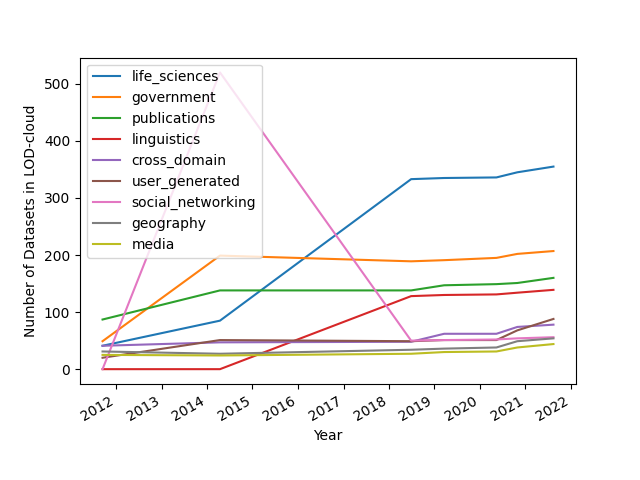
\includegraphics[width=0.7\textwidth]{figures/lod-cloud-change}
        \caption{Change in the number of datasets in the LOD-cloud over the recent years by domain.}
        \label{fig:lod-cloud-change}
    \end{figure}

    \subsection{Maintenance}
    Another aspect of LSLOD currency is whether the datasets are being actively maintained.
    Figure~\ref{fig:bioportal-maintenance} illustrates the time that has passed since the last time that ontologies in BioPortal have been updated.
    There are some ontologies that haven't been updated in several years, but overall it shows that much more both small and large ontologies have seen an update in the last year.

    \begin{figure}[ht]
        \centering
        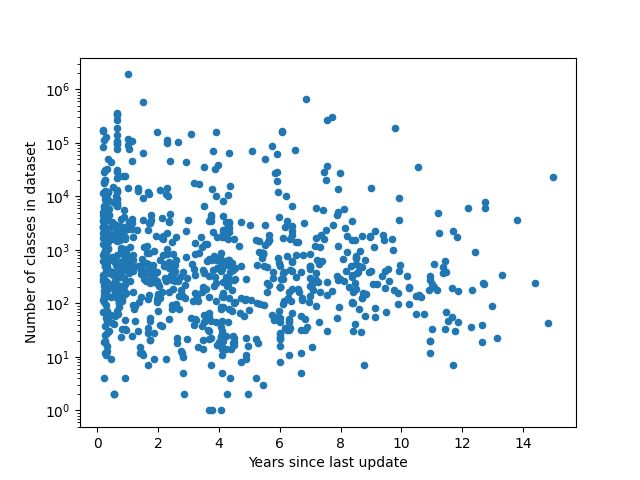
\includegraphics[width=0.7\textwidth]{figures/bio-portal-maintenance}
        \caption{Years since last update of datasets in BioPortal by number of classes in each dataset.}
        \label{fig:bioportal-maintenance}
    \end{figure}

    Unfortunately, it's different for the datasets provided by Bio2RDF and the EBI RDF Platform.
    Bio2RDF was last updated in 2014~\citep{Bio2RDF_Github} and the EBI RDF Platform has seen its last update in 2017 and states on its webpage that the project has run out of funding\footnote{New RDF platform released!, \url{https://www.ebi.ac.uk/rdf//2017/07/10/first-post/}, (Accessed on 01/09/2022)}.


    Please note that the first paragraph of a section or subsection is
    not indented.
    The first paragraph that follows a table, figure,
    equation etc. does not need an indent, either.

    Subsequent paragraphs, however, are indented.

    \subsubsection{Sample Heading (Third Level)} Only two levels of
    headings should be numbered. Lower level headings remain unnumbered;
    they are formatted as run-in headings.

    \paragraph{Sample Heading (Fourth Level)}
    The contribution should contain no more than four levels of
    headings. Table~\ref{tab1} gives a summary of all heading levels.

    \begin{table}
        \caption{Table captions should be placed above the
        tables.}\label{tab1}
        \begin{tabular}{|l|l|l|}
            \hline
            Heading level     & Example                                          & Font size and style \\
            \hline
            Title (centered)  & {\Large\bfseries Lecture Notes}                  & 14 point, bold      \\
            1st-level heading & {\large\bfseries 1 Introduction}                 & 12 point, bold      \\
            2nd-level heading & {\bfseries 2.1 Printing Area}                    & 10 point, bold      \\
            3rd-level heading & {\bfseries Run-in Heading in Bold.} Text follows & 10 point, bold      \\
            4th-level heading & {\itshape Lowest Level Heading.} Text follows    & 10 point, italic    \\
            \hline
        \end{tabular}
    \end{table}


    \noindent Displayed equations are centered and set on a separate
    line.
    \begin{equation}
        x + y = z
    \end{equation}
    Please try to avoid rasterized images for line-art diagrams and
    schemas. Whenever possible, use vector graphics instead (see
    Fig.~\ref{fig1}).

    \begin{figure}
        \caption{A figure caption is always placed below the illustration.
        Please note that short captions are centered, while long ones are
        justified by the macro package automatically.} \label{fig1}
    \end{figure}

    \begin{theorem}
        This is a sample theorem. The run-in heading is set in bold, while
        the following text appears in italics. Definitions, lemmas,
        propositions, and corollaries are styled the same way.
    \end{theorem}
%
% the environments 'definition', 'lemma', 'proposition', 'corollary',
% 'remark', and 'example' are defined in the LLNCS documentclass as well.
%
    \begin{proof}
        Proofs, examples, and remarks have the initial word in italics,
        while the following text appears in normal font.
    \end{proof}
    For citations of references, we prefer the use of square brackets
    and consecutive numbers. Citations using labels or the author/year
    convention are also acceptable. The following bibliography provides
    a sample reference list with entries for journal
%
% ---- Bibliography ----
%
% BibTeX users should specify bibliography style 'splncs04'.
% References will then be sorted and formatted in the correct style.
%
    \bibliographystyle{technopress}
    \bibliography{references}
%
\end{document}
